\appendix
\chapter*{Appendix}

\section{Code for creating a Hierarchical Injector in an Angular Elements component}

\begin{lstlisting}[language={JavaScript},caption={The code for creating a Hierarchical Injector in an Angular Elements component},label={lst:appendix:hierarchical-injectors}]
	// This injector is provided by Angular to the root module
	var rootInjector = ...;
	
	// Create a fake injector
	const _MOCK_INJECTOR = {
		get() {
			return {
				run() {},
				resolveComponentFactory() {
					return {
						inputs: [],
					};
				},
			};
		},
	};
	
	// Extract defualt NgElementStrategy
	function getDefaultNgElementStrategy() {
		const customElement = createCustomElement(EmptyAngularComponent, {
			injector: _MOCK_INJECTOR,
		});
		const proto = customElement.prototype;
		const strategyInstance = proto.ngElementStrategy;
		return strategyInstance.constructor;
	
	}
	
	// Get the NodeInjector class
	function getNgInjectorClass(rootInjector) {
		const componentFactory = rootInjector.get(ComponentFactoryResolver).resolveComponentFactory(EmptyAngularComponent);
		const componentInstance = componentFactory.create(rootInjector, []);
		return componentInstance.injector.constructor
	}
	
	// Get given HTML element's nodeinjector
	function getNodeInjector(rootInjector, host) {
		const hostContext = host.__ngContext__;
		const lView = hostContext.lView;
		const tNode = lView[1].data[hostContext.nodeIndex];
		const NodeInjectorClass = getNgInjectorClass(rootInjector);
		return new NodeInjectorClass(tNode, lView);
	}
	
	// Create a custom NgElementStrategy
	class CustomNgElementStrategy extends getDefaultNgElementStrategy() {
		originalInjector = this.injector;
	
		connect(element): void {
			if (this.injector === this.originalInjector) {
				const localRoot = element.getRootNode();
				const host = localRoot.host;
				const nodeInjector = getNodeInjector(rootInjector, host);
	
				this.injector = Injector.create({
					providers: [],
					parent: nodeInjector,
				});
	
				return this._connectSuperWithDelayedInit(element);
			}
	
			return super.connect(element);
		}
	}
	
	// Create a custom NgElementStrategyFactory that creates
	// instances of our custom NgElementStrategy
	class CustomNgElementStrategyFactory {
		constructor(
			private _StrategyConstructor,
			component,
			injector,
		) {
			this.componentFactory = injector
				.get(ComponentFactoryResolver)
				.resolveComponentFactory(component);
		}
	
		create(injector) {
			return new this._StrategyConstructor(this.componentFactory, injector);
		}
	}
	
	// Provide the CustomNgElementStrategyFactory to the createCustomElement
	// function and create a new Web Component
	const WebComponent = createCustomElement(AngularComponent, {
		injector: rootInjector,
		strategyFactory: new CustomNgElementStrategyFactory(
			CustomNgElementStrategy,
			AngularComponent,
			rootInjector
		)
	})
		\end{lstlisting}

	\section{Code used for render-on-demand functions for various JS frameworks}

	\begin{lstlisting}[language={JavaScript},caption={The render-on-demand function in ReactJS},label={lst:appendix:react-set-visible}]
		const App = () => {
			const [ visibleComponent, setVisibleComponent ] = React.useState(null);
		
			window.setVisibleComponent = (componentName) => {
				setVisibleComponent(componentName);
			}
		
			return (
				{ visibleComponent === 'Button' && <Button />}
			)
		};
		\end{lstlisting}
		
		\begin{lstlisting}[language={HTML},caption={The render-on-demand function in Angular (HTML file)},label={lst:appendix:angular-set-visible-html}]
		<button *ngIf="visibleComponent == 'Button'" />
		\end{lstlisting}
		
		\begin{lstlisting}[language={JavaScript},caption={The render-on-demand function in Angular (JavaScript file)},label={lst:appendix:angular-set-visible-js}]
		@Component({
			...
		})
		export class AppComponent {
			constructor(private _cd: ChangeDetectorRef) {
				window.setVisibleComponent = (componentName) => {
					this.visibleComponent = componentName;
					this._cd.detectChanges();
				}
			}
		
			public visibleComponent = null;
		}
		\end{lstlisting}
		
		\begin{lstlisting}[language={HTML},caption={The render-on-demand function in Svelte},label={lst:appendix:svelte-set-visible}]
		<script>
			window.setVisibleComponent = (componentName) => {
				visibleComponent = componentName;
			}
		
			let visibleComponent = null;
		</script>
		
		{#if visibleComponent === 'Button'}
			<Button />
		{/if}
		\end{lstlisting}
		
		\begin{lstlisting}[language={JavaScript}, caption={The render-on-demand function in Web Components},label={lst:appendix:web-components-set-visible}]
		window.setVisibleComponent = (componentName) => {
			if (componentName === 'Button') {
				document.body.appendChild(document.createElement('x-button'));
			}
		}
		\end{lstlisting}

	\section{Render times for all components}

	\begin{figure}[h]
		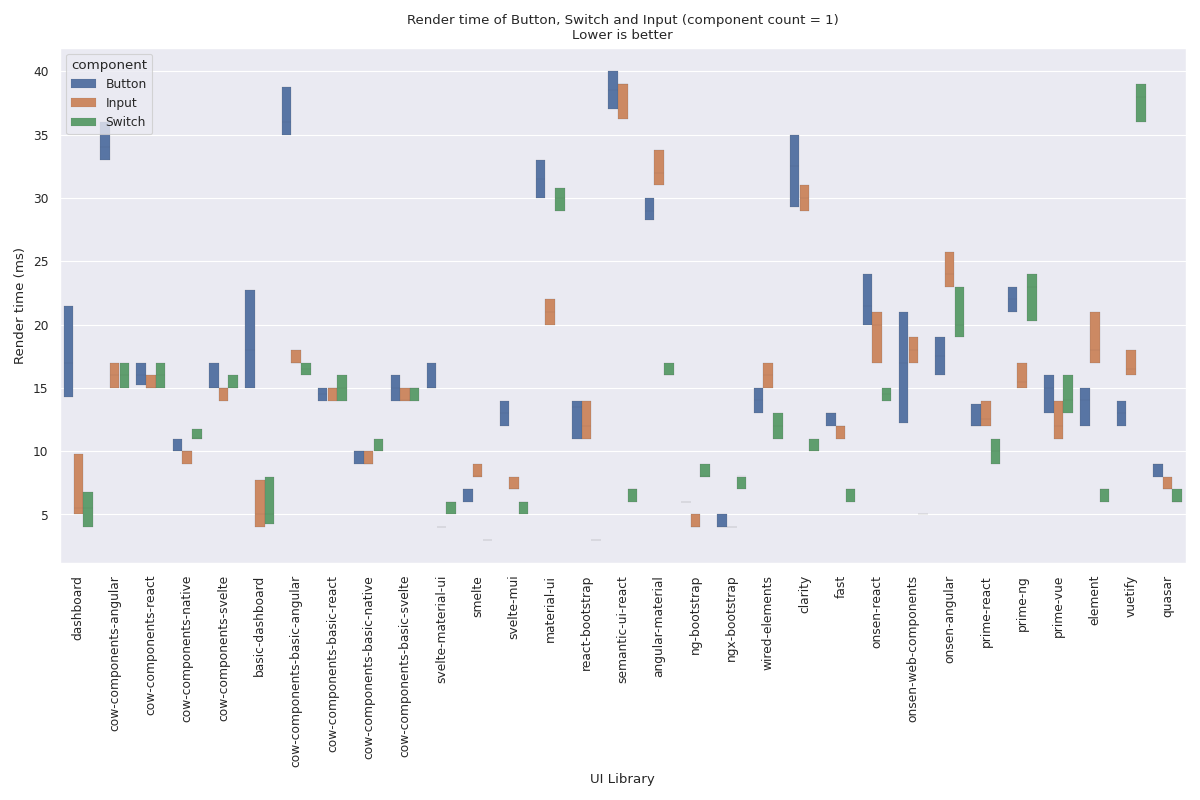
\includegraphics[width=\columnwidth]{plots/render-time-all-big-1.png}
		\caption{Render times of a single Button, Switch, or Input component}
		\label{fig:appendix:render-time-cow-1}
		\centering
	\end{figure}

	\begin{figure}[h]
		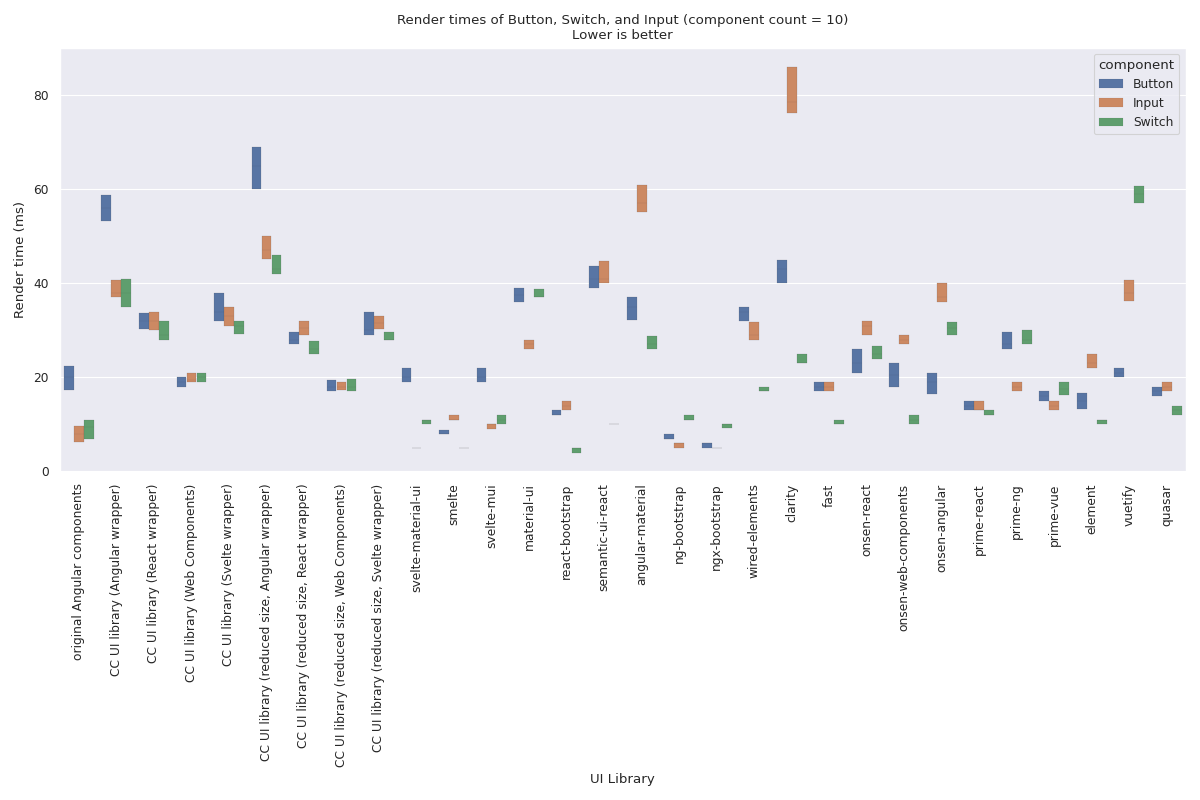
\includegraphics[width=\columnwidth]{plots/render-time-all-big-10.png}
		\caption{Render times of ten Button, Switch, or Input components}
		\label{fig:appendix:render-time-cow-10}
		\centering
	\end{figure}

	\begin{figure}[h]
		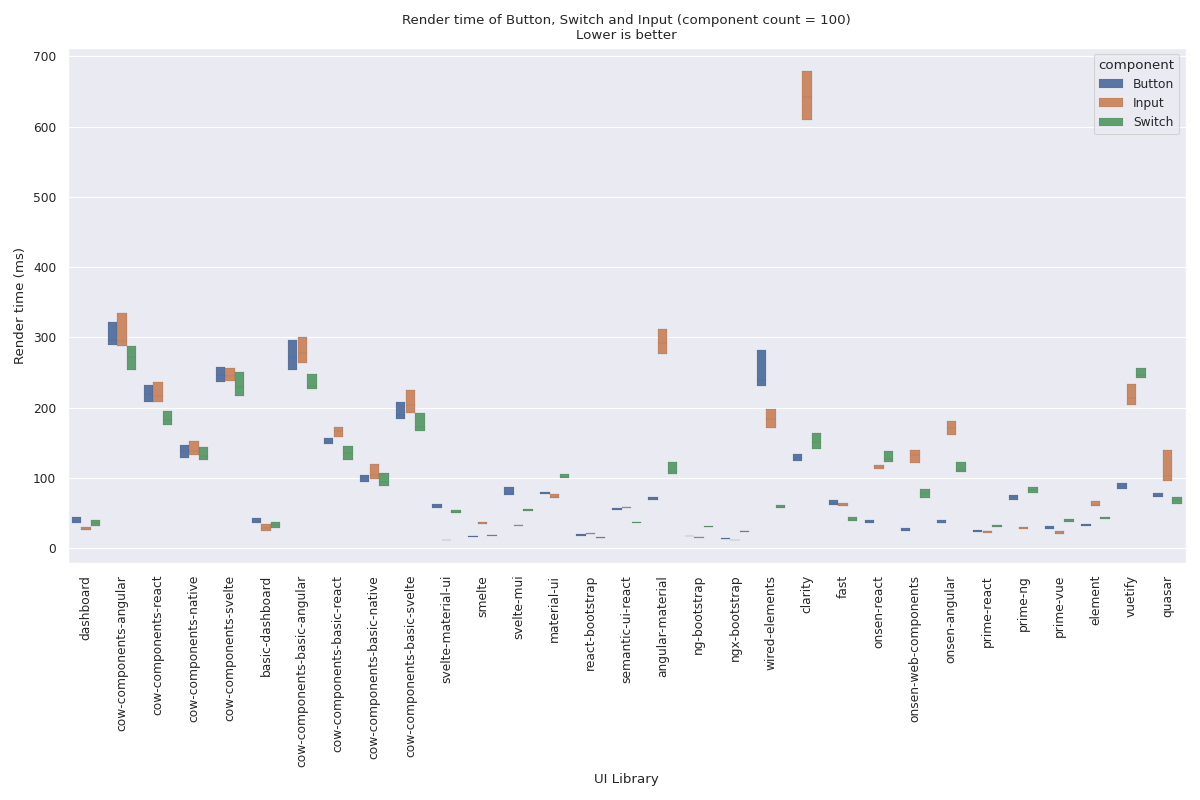
\includegraphics[width=\columnwidth]{plots/render-time-all-big-100.png}
		\caption{Render times of one hundred single Button, Switch, or Input components}
		\label{fig:appendix:render-time-cow-100}
		\centering
	\end{figure}